\section{Web hacking}

\subsection{Unicorn 1 (100p)}
\subsection{Tricky login (100p)}

\newpage
\subsection{Order a Unicorn (100p)}
\addtocounter{points}{100}
Do you want to order a Unicorn?
\\Well, let's try it: \url{http://julie2.hackingarena.no:804}

\textbf{Solution:}\\
First I used the php filter \texttt{php://filter/convert.base64-encode/resource=index.php} to get the base64 encoded source code of the index.php file. 

\begin{center}
    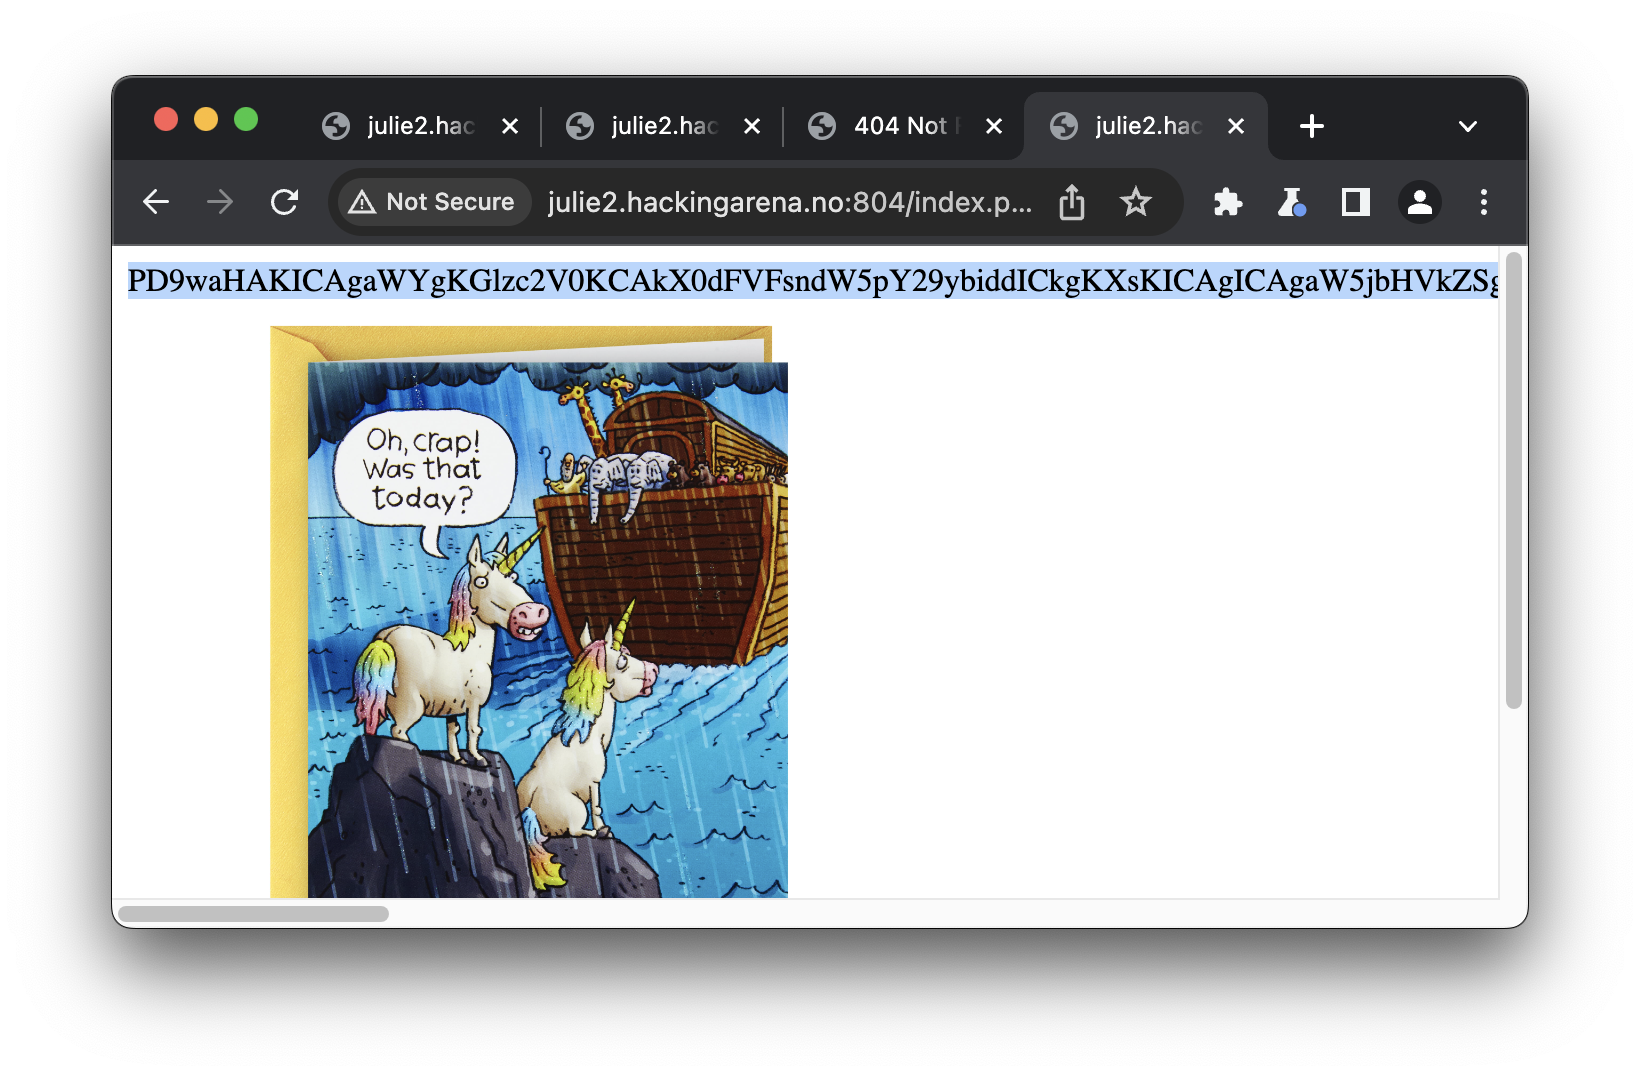
\includegraphics[width=12cm]{img/Web hacking/Order a Unicorn/Screenshot 2023-11-24 at 12.54.35.png}
\end{center}

Then I decoded it and found the following code:

\begin{center}
    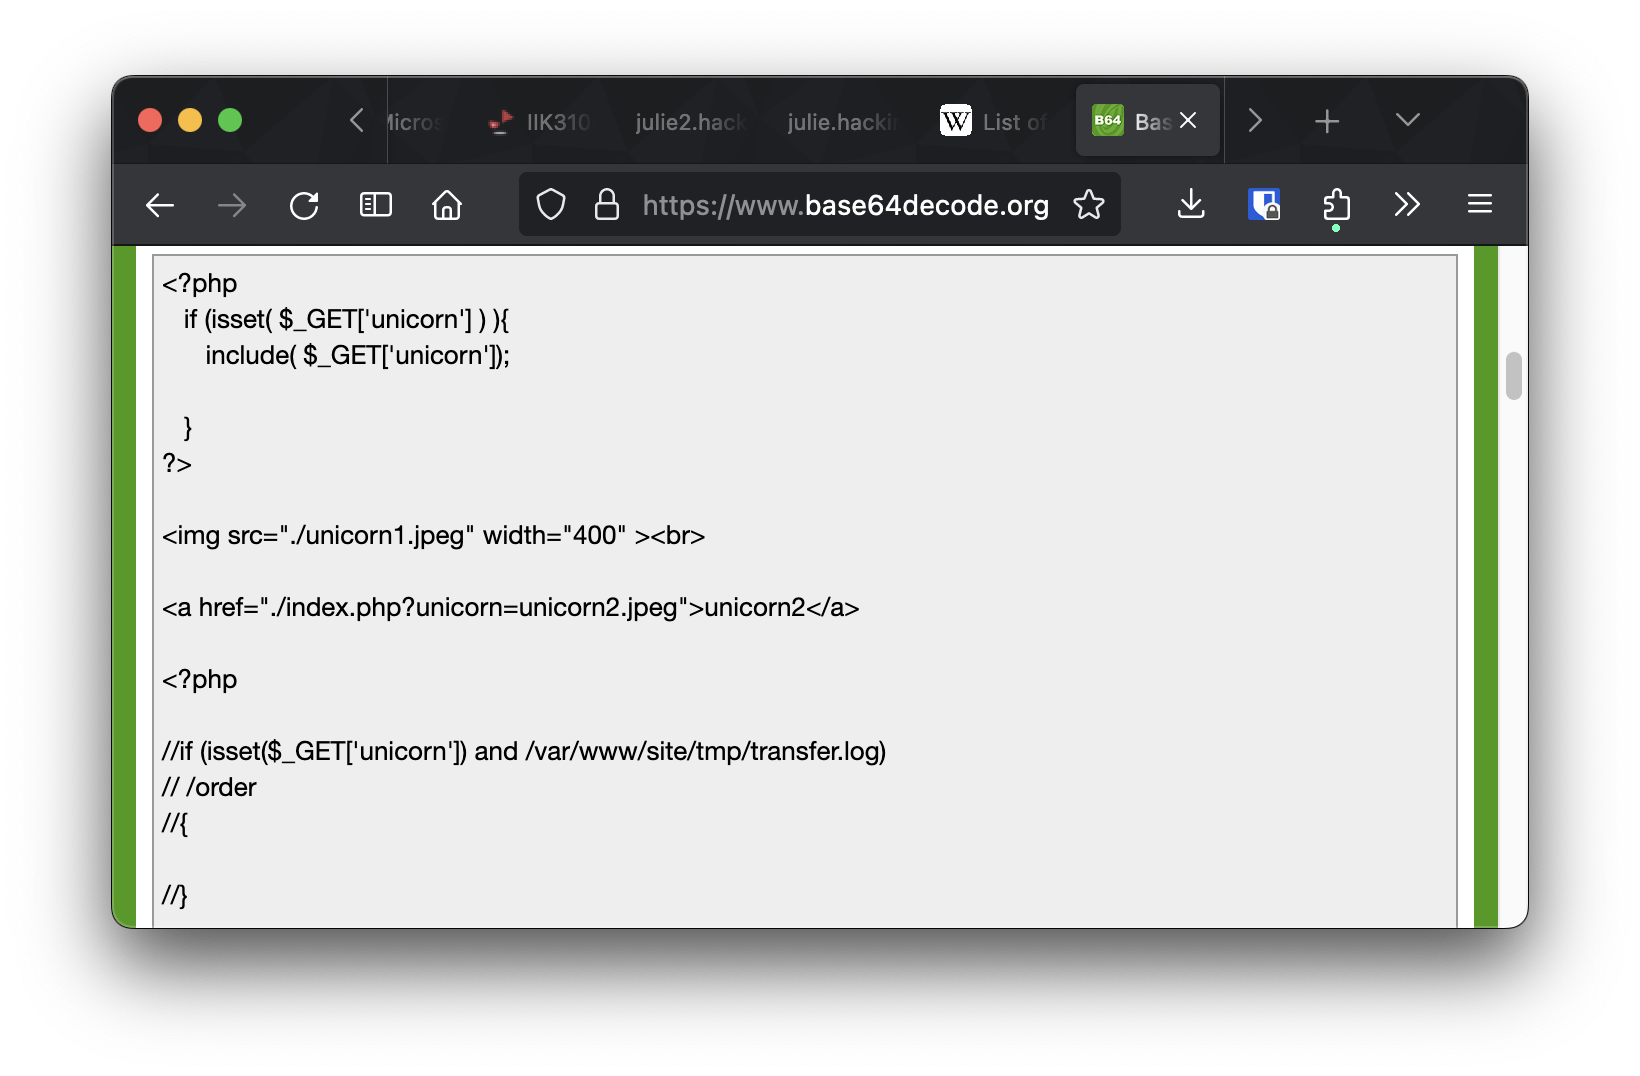
\includegraphics[width=12cm]{img/Web hacking/Order a Unicorn/Screenshot 2023-11-24 at 12.54.54.png}
\end{center}

I then looked at the \texttt{/var/www/site/tmp/transfer.log} that was revealed by the source code and found the following stride payment records:

\begin{center}
    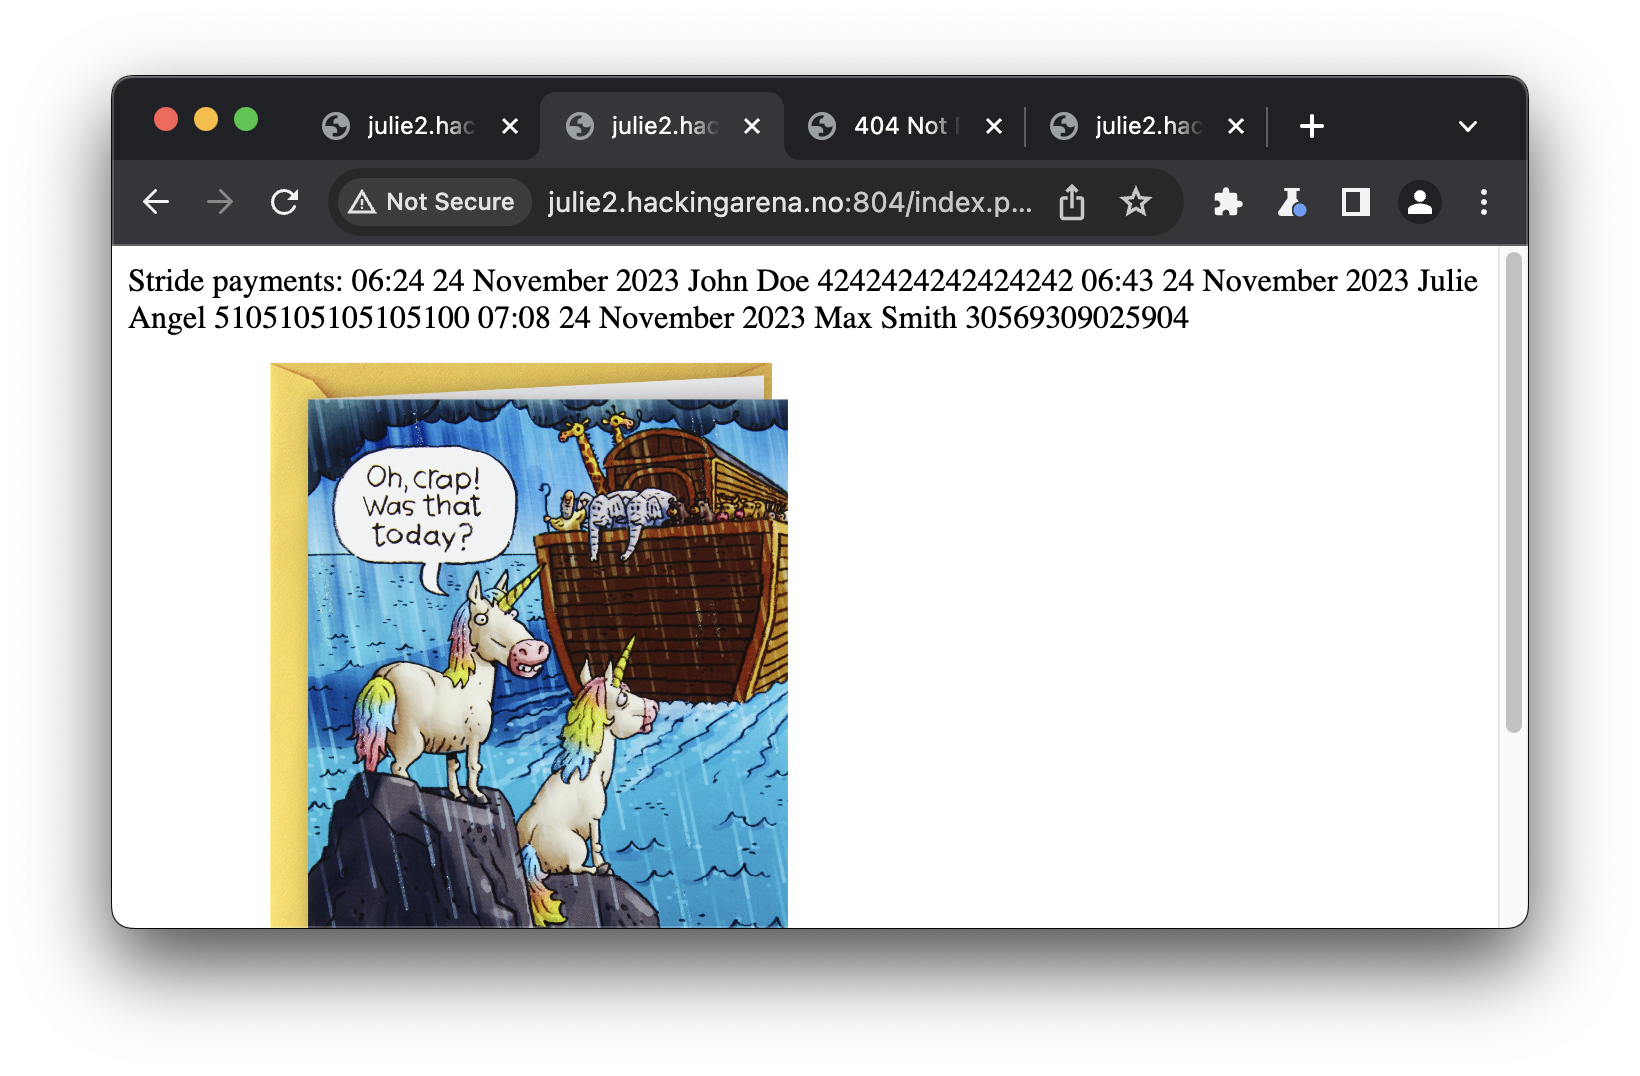
\includegraphics[width=14cm]{img/Web hacking/Order a Unicorn/Screenshot 2023-11-24 at 12.55.13.png}
\end{center}

I then when to the \texttt{/order} page and tried to order a unicorn with the card numbers from the stride payment records. But since none of them worked I started looking for example card numbers online and found a list from paypal test credit cards.

\begin{center}
    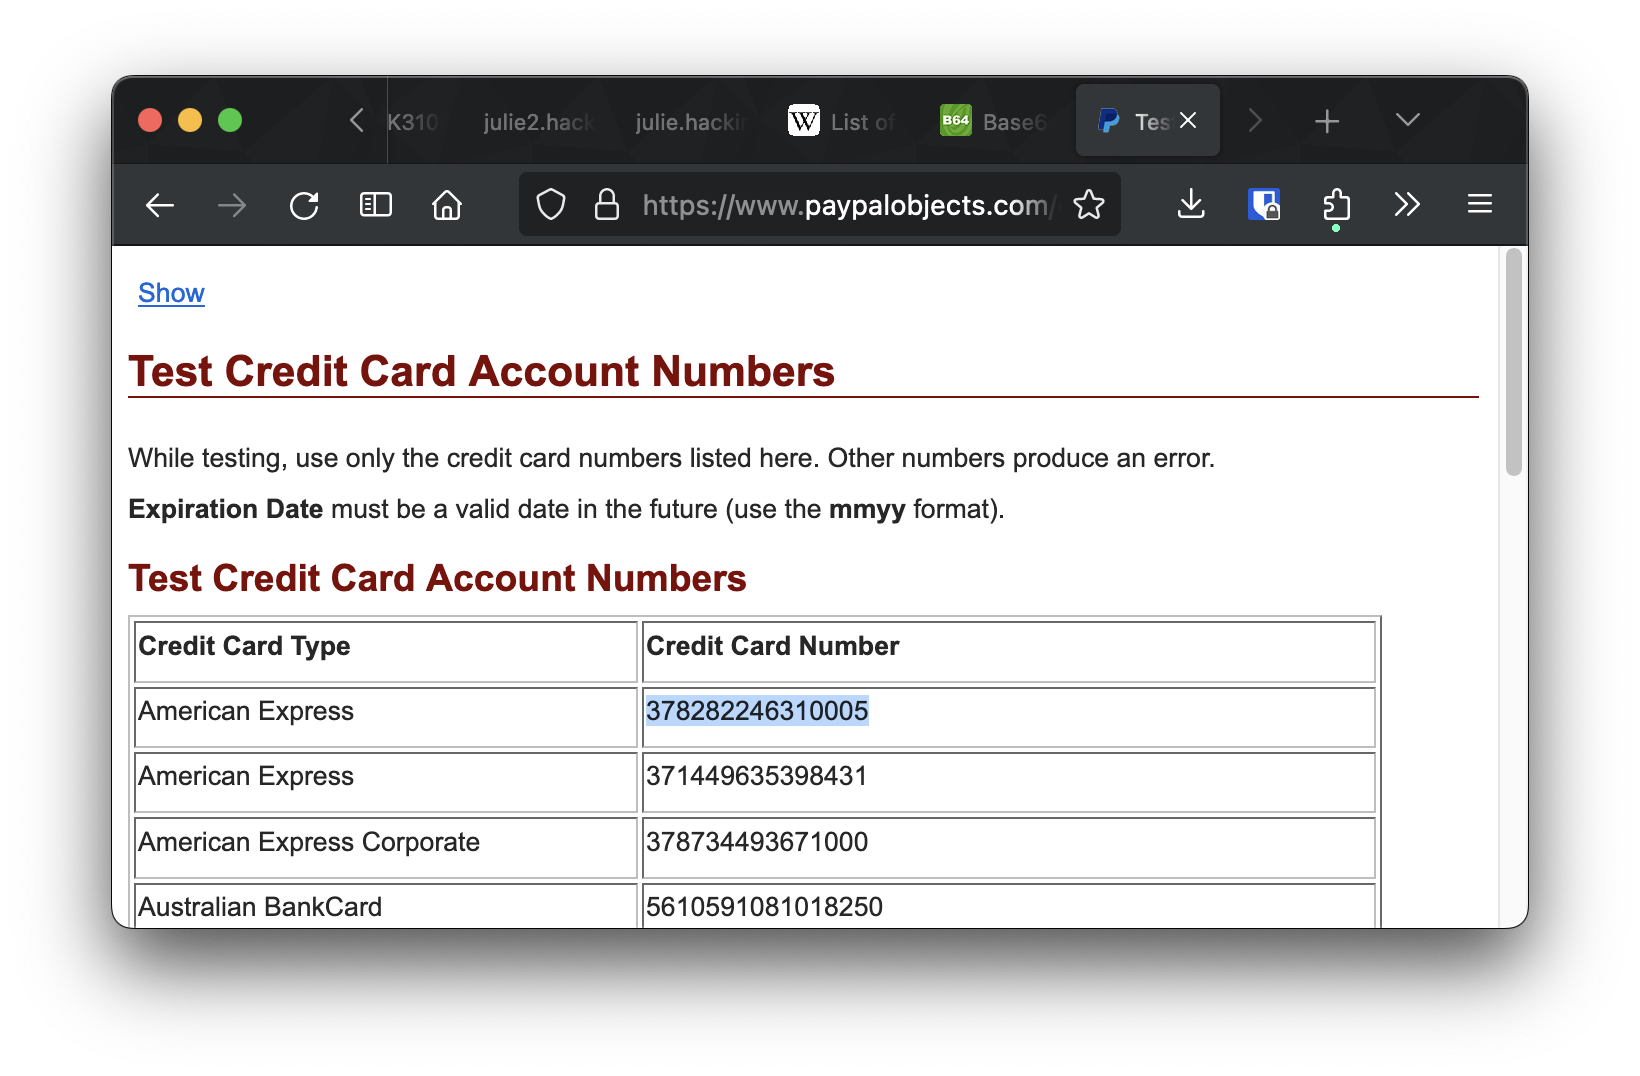
\includegraphics[width=15cm]{img/Web hacking/Order a Unicorn/Screenshot 2023-11-24 at 12.55.43.png}
\end{center}

I then tried to order a unicorn with the card number \texttt{378282246310005}...

\begin{center}
    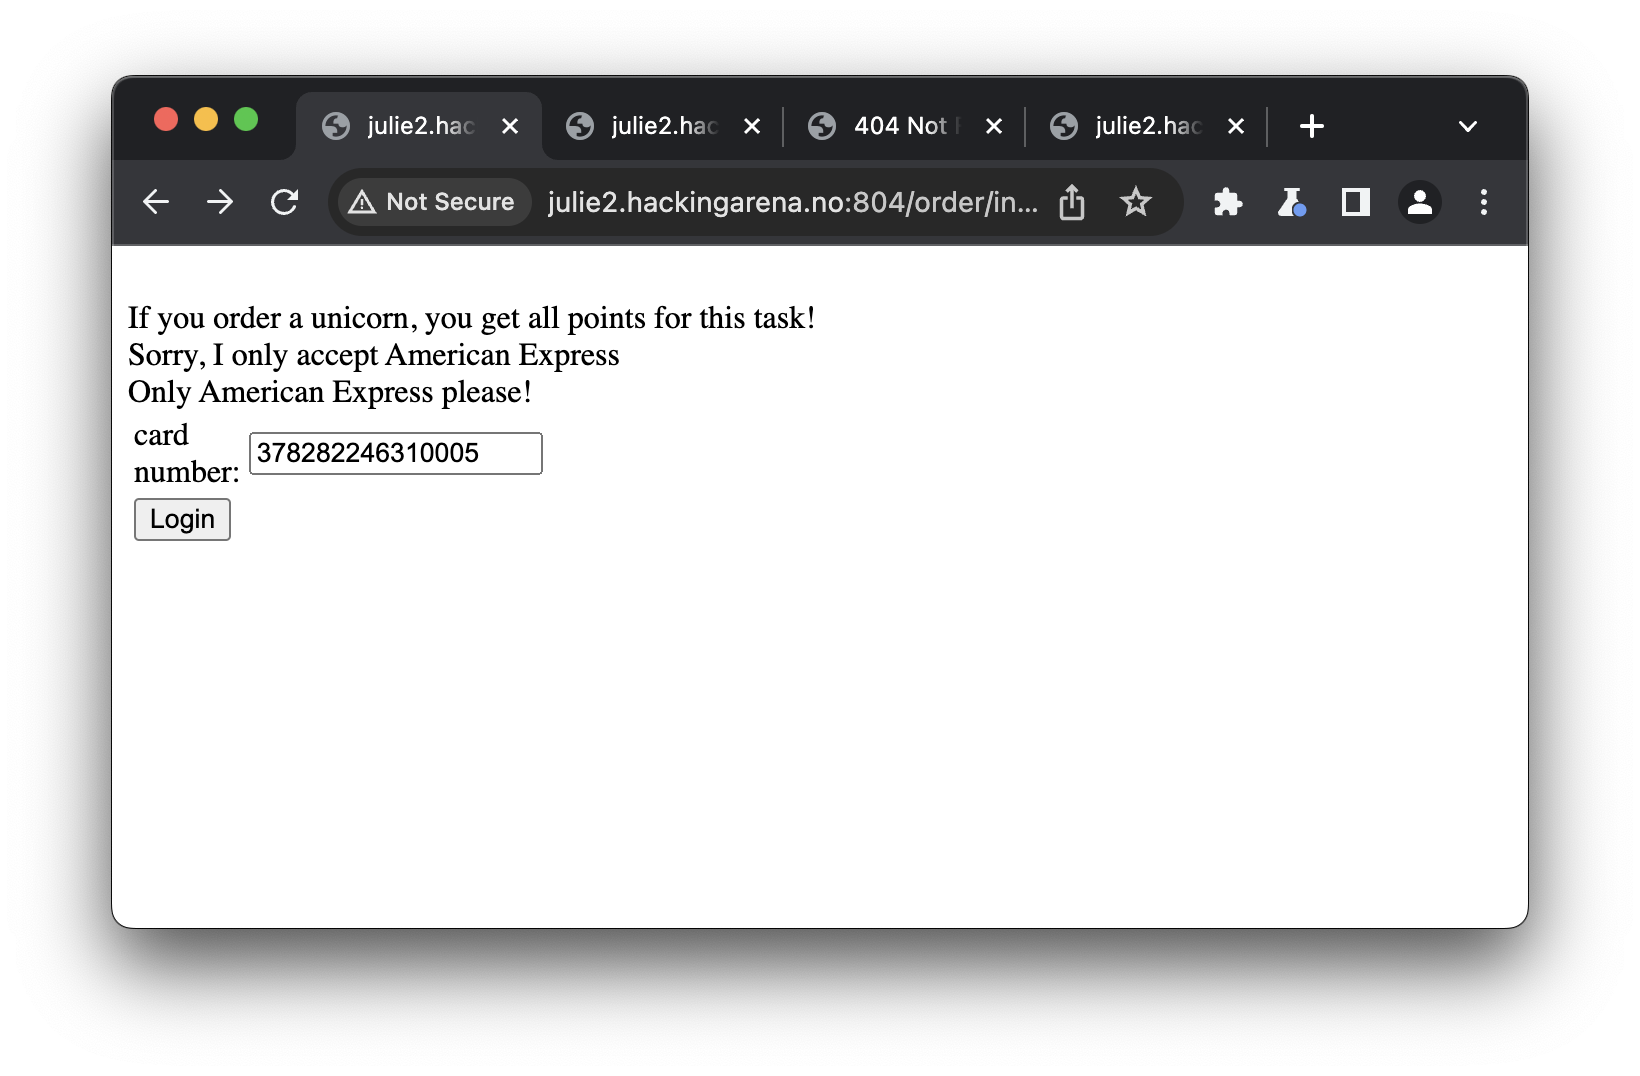
\includegraphics[width=15cm]{img/Web hacking/Order a Unicorn/Screenshot 2023-11-24 at 12.55.22.png}
\end{center}

...and got the flag.

\begin{center}
    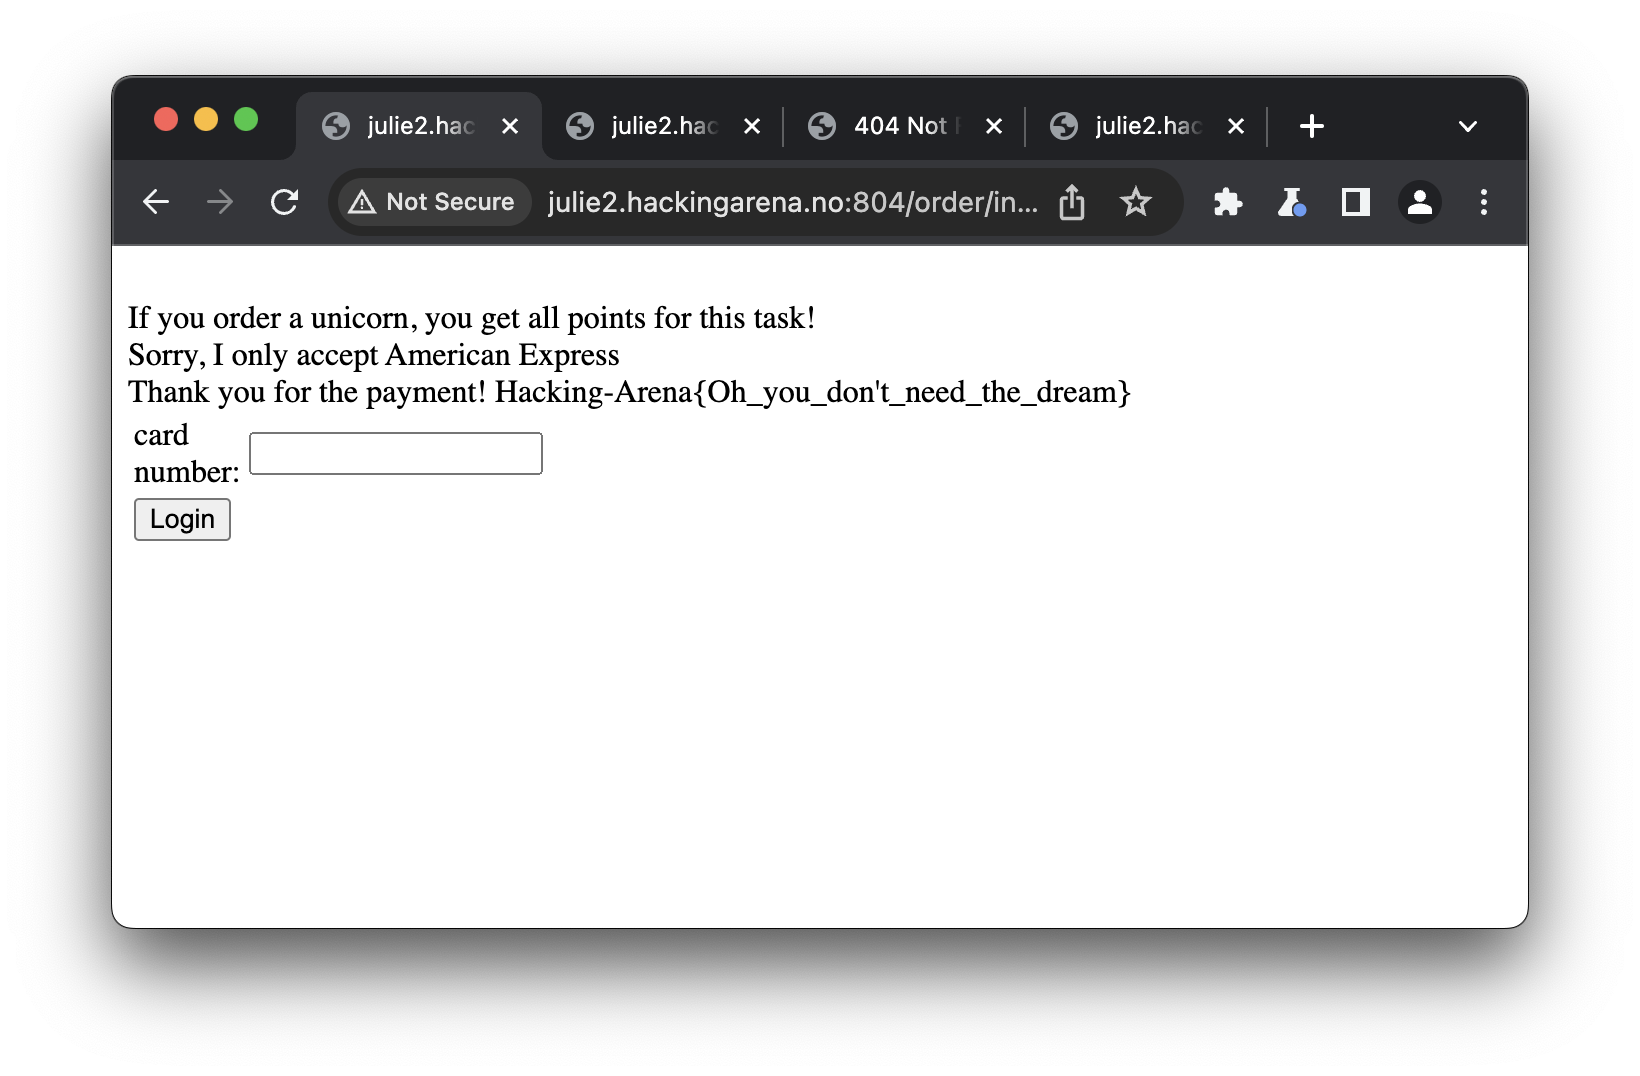
\includegraphics[width=15cm]{img/Web hacking/Order a Unicorn/Screenshot 2023-11-24 at 12.55.26.png}
\end{center}